%!TEX program = lualatex
\documentclass[10pt, a4paper]{article}
\usepackage{fontspec}
\usepackage{polyglossia}
\setdefaultlanguage{danish}
\usepackage[left=1.3cm, right=1.3cm, vmargin=1.25cm, noheadfoot, marginparwidth=0cm]{geometry} % sidemargener
%\usepackage[final]{microtype} % the art of enhancing the appearance and readability of a document
\usepackage{titlesec}
\usepackage{color}
\usepackage{grid-system}
\usepackage{amssymb}
\usepackage[svgnames]{xcolor}
\usepackage{hyperref} % hyper links
\usepackage{marvosym} % symboler for telefon, email m.v.
\usepackage{nopageno} % undlad side-nummer
%\usepackage{coffee4}
\usepackage{setspace}

\definecolor{linkColor}{HTML}{408AF8}
\definecolor{bulletColor}{HTML}{CAA239} % 1D8BB9 336F3A

\setmainfont[Ligatures=TeX]{akkurat}[
  BoldFont = Helvetica Neue Bold]

\setlength{\parindent}{0pt}
\titleformat{\section}{\bfseries\Large\scshape\raggedright\color{bulletColor}}{}{0em}{}

\newcommand*{\opgave}[1]{\(\textcolor{bulletColor}{\blacksquare}\) #1\\}

\hypersetup{
     colorlinks   = true,
     citecolor    = linkColor,
     urlcolor     = linkColor
}

\newcommand*{\contactinfo}[7]{
\begin{minipage}[t][1.5cm][t]{.5\textwidth}
\begin{tabular}{@{}l@{}} % The @{} at start and end removes the outer padding
{\huge\scshape\bfseries #1} \\[2ex]
{\Large\scshape #2}
\end{tabular}
\end{minipage}
\hfill
\begin{minipage}[t][1.5cm][t]{.5\textwidth}
\hfill
\texttt{
\begin{tabular}{l}
#3 \\
#4 \\[1ex]
\Telefon{ #5}\\
\Letter{ #6}\\
\Mundus{ #7}
\end{tabular}
}
\end{minipage}
}

\newcommand*{\worktitle}[1]{#1}

\newcommand*{\kursus}[2]
{
    \begin{Row}%
      \begin{Cell}{1}
        #1
      \end{Cell}
      \begin{Cell}{3}
        #2
      \end{Cell}
    \end{Row}
}

\newcommand*{\kompetence}[2]
{
    \begin{Row}%
      \begin{Cell}{1}
        #1
      \end{Cell}
      \begin{Cell}{3}
        #2
      \end{Cell}
    \end{Row}
}

\newcommand*{\uddannelse}[3]
{
    \begin{Row}%
      \begin{Cell}{1}
        \worktitle{#1} \\
        #2 % chktex 8
      \end{Cell}
      \begin{Cell}{3}
        #3
      \end{Cell}
    \end{Row}
}

\newcommand*{\job}[5]
{
\begin{Row}%
  \begin{Cell}{1}
    \textbf{#1} \\ [1ex]
    #2 \\
    #3
  \end{Cell}
  \begin{Cell}{3}
    #4 \\ [1ex] #5
  \end{Cell}
\end{Row}
}


\begin{document}
%===============================================================================
% Kontakt info
%===============================================================================
\begin{tabular}{@{}p{10cm} p{5cm} p{2.5cm}@{}}
    \vspace{0pt}
    {\LARGE\bfseries C}{\Large\bfseries ARSTEN }{\LARGE\bfseries J}{\Large\bfseries ØRGENSEN}
    
    {\Large\bfseries S}{\large\bfseries OFTWAREUDVIKLER}

    Arkitektur, data og analyse
    &
    \vspace{0pt} 
    Badstuestræde 18D 1. th 
    
    1209 København K 

    \Telefon{ 29712097}

    \Letter{ \href{mailto:carstenj@gmail.com}{carstenj@gmail.com}}
    
    \Mundus{ \href{https://carsten-j.github.io/}{https://carsten-j.github.io/}}
    &
    \vspace{0pt}
    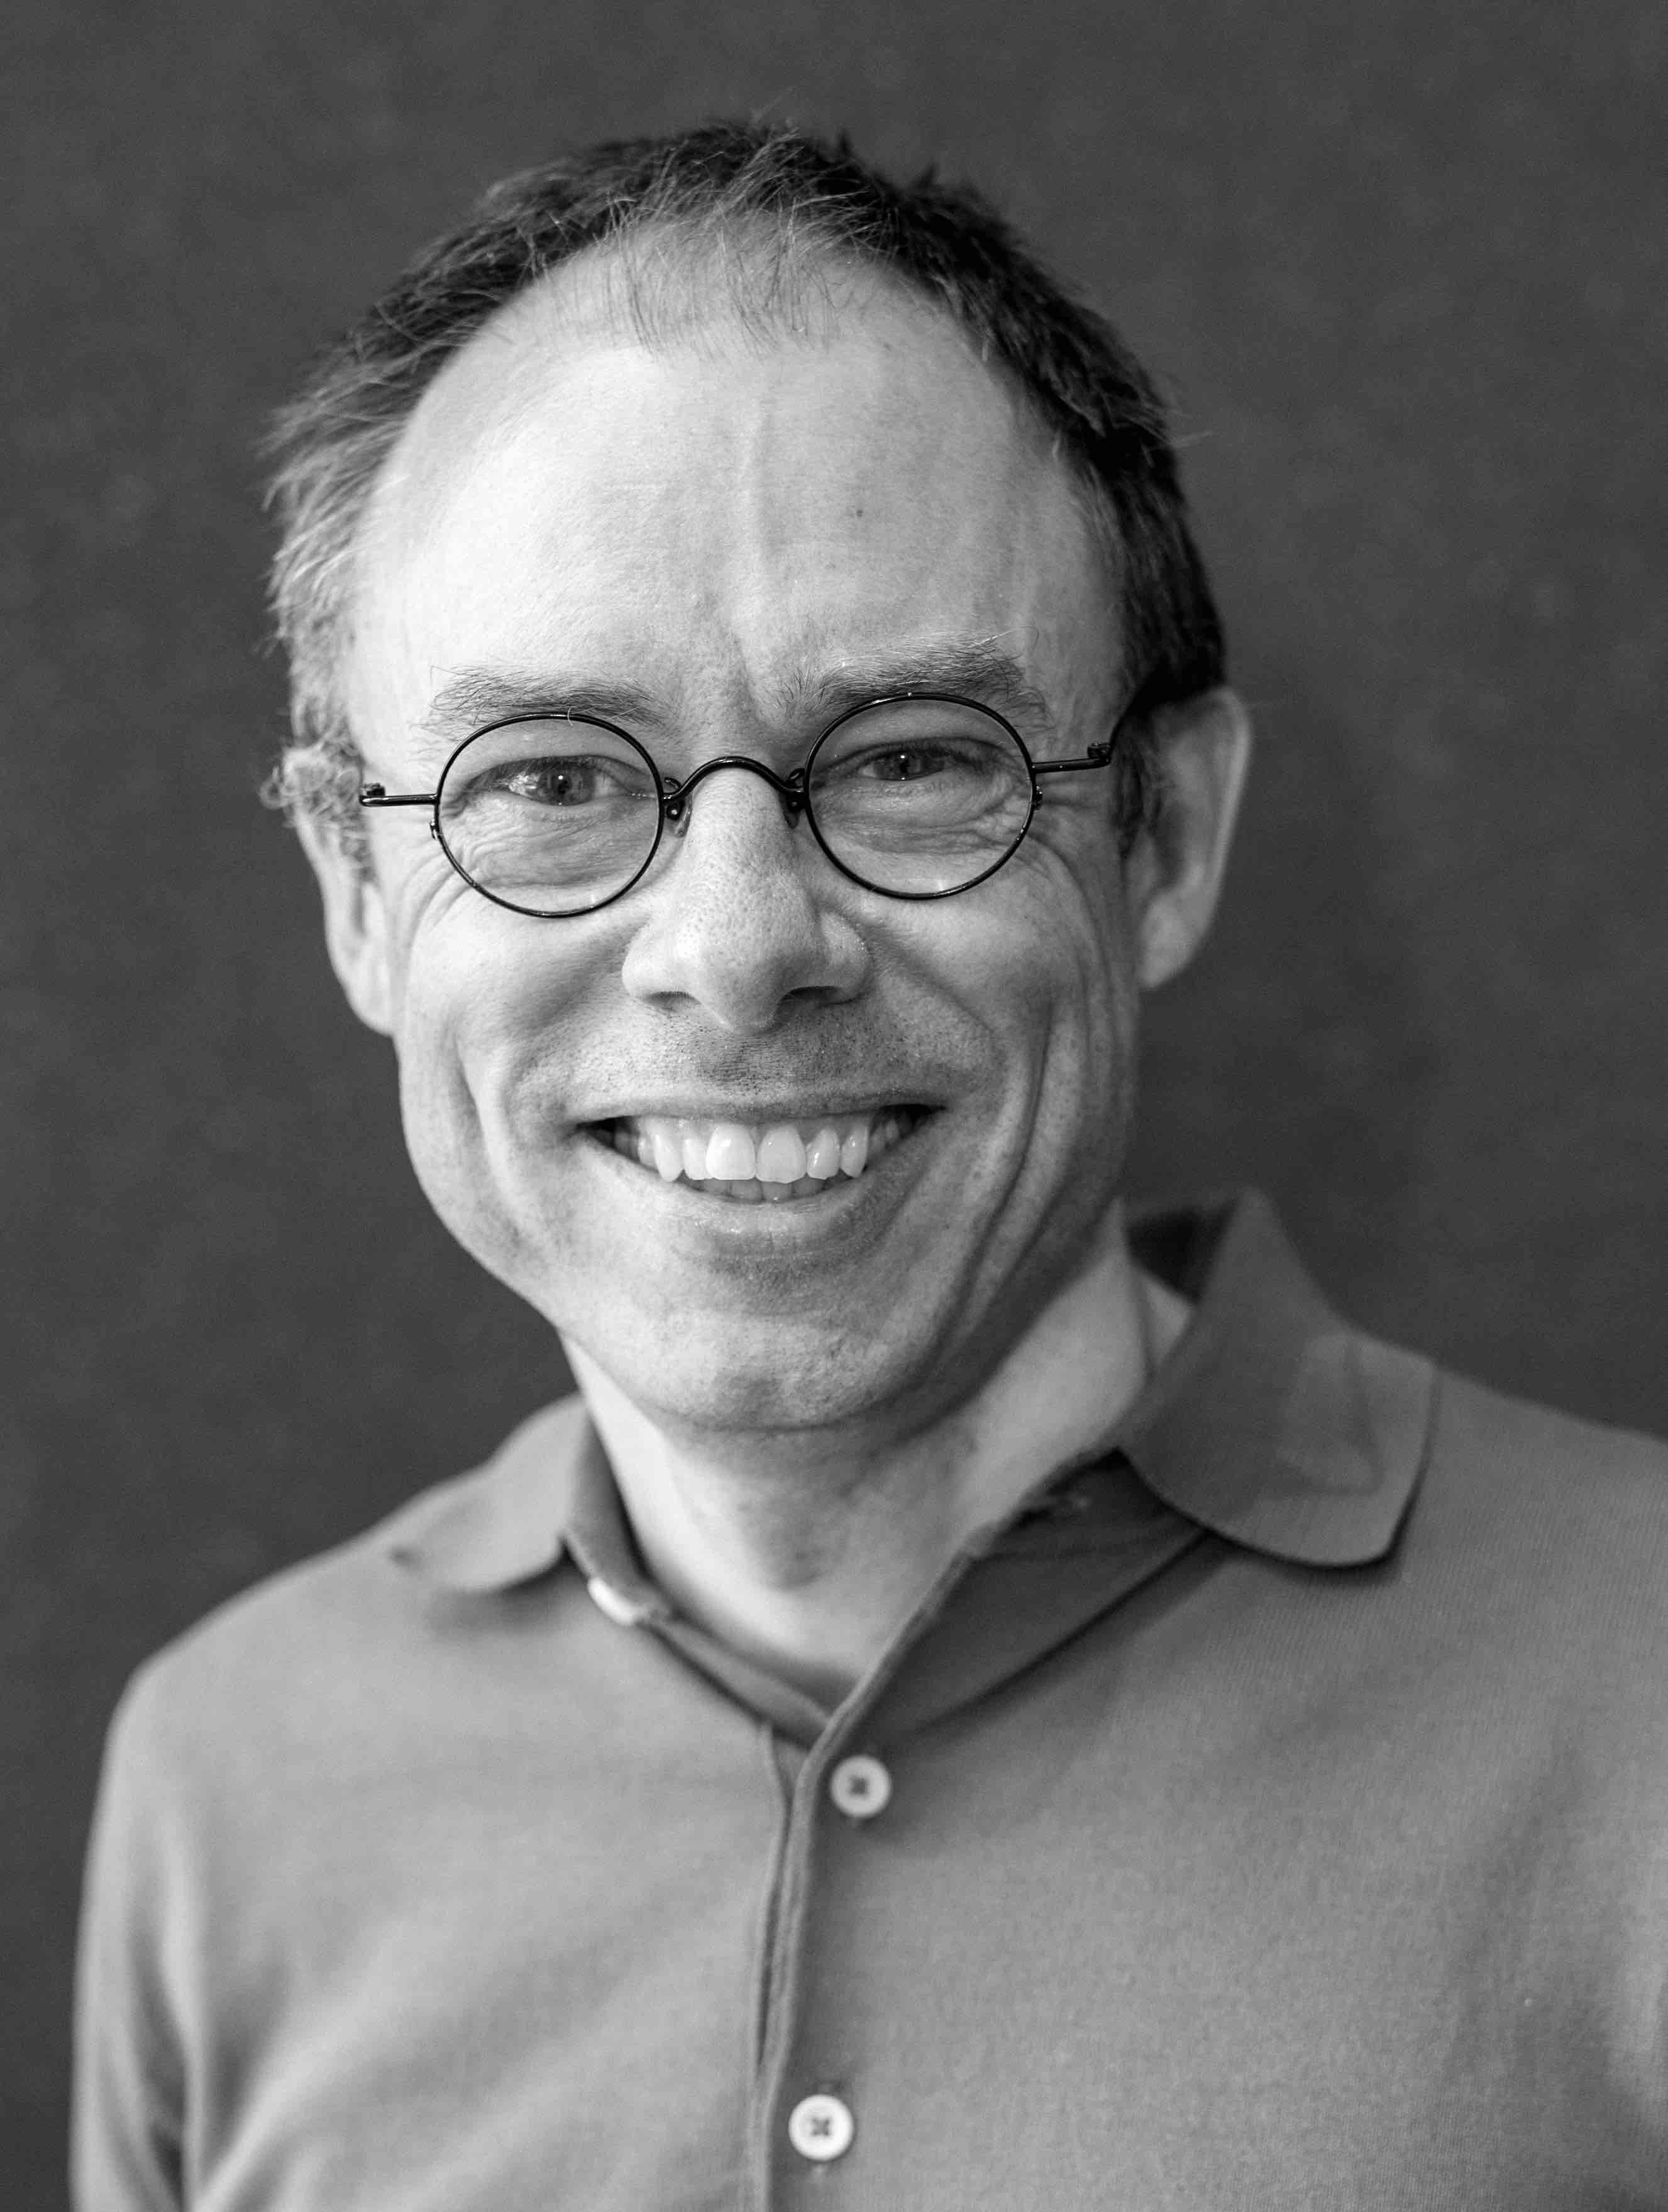
\includegraphics[width=0.1\textwidth]{carsten}
\end{tabular}
%==============================================================================
% Introduktion
%==============================================================================

%\section{Kort fortalt}
%25+ års erfaring med professionel software udvikling af large scale systemer primært til den finansielle sektor. Erfaring med software indenfor områderne finans, optimering, supply chain management og telekommunikation. Omfattende forretningsviden på områderne pension og livsforsikring (7 år), finans, bank og capital markets (13 år) samt ERP systemer (5 år). Mit kendetegn er levering til tiden i den ønskede kvalitet, mens min største styrke er at kunne fungere som bindeled mellem forretning og udvikling.

%==============================================================================
% Erhvervserfaring
% titel, virksomhed, periode, beskrivelse, liste af opgaver
%==============================================================================
\section{Erhvervserfaring}

\job{Senior Software Konsulent}{BlueFragments}{Okt 2021 --}
{I rollen som senior konsulent har jeg kundevendte opgaverne, hvor jeg 
}
{
\opgave{har ansvaret for backend udviklingen og deltager i frontend for et moderniseringsprojekt for en telecom kunde}
\opgave{sparring og coaching for junior udviklere}
}

\job{Senior Software Developer}{CBB Mobil}{Maj 2020 -- Sep 2021}
{Ansat i Business Support Software afdeling, hvor vi har ansvaret for en platform som bruges af 650.000 mobilkunder.
}
{
\opgave{opdatering af online betalingsoplevelse med stærk kundeautentifikation under PSD2 regulativ og integration til ny betalingsløsning}
}

\job{Senior Risk Manager}{P+, Pension for \\Akademikere}{Juni 2019 -- April 2020}
{Som senior softwareudvikler indenfor risikostyring udviklede jeg software i Python til}
{
\opgave{visualisering og rapportering af finansielle data}
\opgave{matematiske modeller til finansiel risikostyring (VaR og Solvens II)}
\opgave{opsætning af devops CI/CD pipelines baseret på BitBucket, Bamboo og Docker}
}

\job{Chief Software Engineer}{Danske Bank, C\&I}{Jan 2016 -- Maj 2019}
{Ansat i Derivative Risk and IT, hvor jeg arbejdede med 360-graders udvikling af}
{
\opgave{realtids rapportering til eksterne myndigheder af regulatoriske krav (MiFID II)}
\opgave{eksponering af bankens Post-Trade løsning som SaaS for eksterne kunder}
\opgave{matematiske modeller til finansiel risikostyring (VaR)}
}

\job{Løsningsarkitekt}{Danmarks Nationalbank}{Nov 2014 -- Dec 2015} %chktex 8
{I rollen som løsningsarkitekt var det mit ansvar at}
{
\opgave{sikre den tekniske leverance for det kommende nationale kre\-dit\-re\-gis\-ter med særlig fokus på arkitektur, IT-sikkerhed og datamængder}
\opgave{bidrage til, at Nationalbankens IT-systemer udvikler sig konsistent og i samme retning}
}

\job{Softwareudvikler og \\ arkitekt}{Edlund A/S}{Dec 2008 -- Okt 2014} %chktex 8
{Som softwareudvikler og arkitekt var det min opgave at udvikle software baseret på forsikringsmatematiske principper og}
{
\opgave{sparre med PFA's forretningsanalytikere omkring krav til PFA\(+\) samt udvikle og implementere den overordnede arkitektur og løsning primært omkring Unitlink}
\opgave{deltage i udviklingen af nyt standard rammesystem til Nordea
Liv og Pension}
\opgave{have den daglige kontakt til Skandia og ansvaret for udvikling af deres kundespecifikke ønsker}
}

\job{Softwareudvikler}{Microsoft}{Mar 2003 -- Nov 2008} %chktex 8
{I mine 5 år hos Microsoft arbejdede jeg på tre større projekter, hvor jeg}
{
\opgave{havde ansvaret for front-end delen af en ny ``Sales and Operations Planning'' feature til næste version af AX}
\opgave{havde medansvar i AX-kerneudvikling til Microsoft Dynamics AX 4.0}
\opgave{deltog i udviklingen af innovativt ERP prototype projekt baseret på SOA arkitektur og en rollebaseret konfigurerbar opsætning af forretningsprocesser.}
}

\job{Chief Financial \\ Consultant}{SimCorp}{Okt 2000 -- Feb 2003} %chktex 8
{I den afdeling som har ansvaret for matematisk finansielle beregninger i SimCorp Dimension var det min opgave at}
{
\opgave{deltage i refaktoreringen af beregningsmotoren fra C til C\(++\) med primært ansvar for optimeringsalgoritmer}
\opgave{være ansvarlig for teamets software releases og konfigurationsstyring}
}

\job{Senior Kvantitativ \\ Analytiker}{Nordea Markets}{Okt 1997 -- Sep 2000} %chktex 8
{Som analytiker var jeg med til at}
{
\opgave{udvikle funktionalitet og Excel løsninger til Nordea Analytics platformen}
\opgave{udvikle Markets interne modeller til prepayment- og realkreditmodellering}
\opgave{implementere, teste og konvertere et ældre system til Infinity Financial Technology systemet med ansvar for rentederivater}
}

\job{Softwareudvikler}{SimCorp}{Aug 1995 -- Sept 1997} %chktex 8
{Som software udvikler var det min opgave at deltage i}
{
\opgave{den årlige release af en række Excel add-ins}
\opgave{koordineringen af en tværafdelings udviklingsopgave af modul til Ka\-pi\-tal\-dæk\-nings\-di\-rek\-ti\-vet}
\opgave{udviklingen af matematisk finansielt bibliotek i C med tilhørende unit tests}
}

%===============================================================================
% Uddannelse afsnit
%===============================================================================
\section{Uddannelse}
\uddannelse{Softwareudvikling}{2002 -- 2006}{IT Universitetet. Kurser i database og distribuerede systemer, algoritmer og datastrukturer, programmeringssprog samt avanceret objekt-orienteret programmering} %chktex 8
\\[0.2cm]
\uddannelse{Visiting Member}{1999}{Courant Institute of Mathematical Sciences, New York University. Mathematics of Finance. Vært Marco Avellaneda. Modtager af Andersens Rejselegat for Matematikere}
\\[0.2cm]
%\uddannelse{Erasmus program}{1992 -- 1993}{University of Leeds, England. Anvendt statistik og ikke-kommutativ algebra} %chktex 8
%\\[0.25cm]
\uddannelse{Cand. Scient}{1988 -- 1995}{Københavns Universitet. Hovedfag i matematik og bifag i statistik. Fokusområder: Numerisk analyse og målteori} %chktex 8

%===============================================================================
% Kompetencer
%===============================================================================
\section{Kompetencer}
\kompetence{Programmeringssprog \\ og frameworks}{Produktionserfaring med: Python, C\#, .NET Core/Framework, Akka.NET, WPF, WCF, C\(++\) og C. Derudover kendskab til F\#, Java, Scala og R}
\\[0.2cm]
\kompetence{Web}{ASP.NET Core, Blazor, MVC, Web API, JavaScript}
\\[0.2cm]
\kompetence{Cloud}{Primært Microsoft Azure og i mindre grad Google Cloud}
\\[0.2cm]
\kompetence{Data systemer}{SQL Server, MongoDB, Redis, RabbitMQ og Kafka}
\\[0.2cm]
\kompetence{DevOps tools}{Docker, Ansible, Elastic, Kibana, InfluxDB, Grafana, Octopus, 
GoCD, Git, Mercurial, GitHub, TFS, Vic\-tor\-Ops, Icinga2, Bamboo, BitBucket}

%===============================================================================
% Kurser
%===============================================================================
\begin{onehalfspacing}
\section{Nyere udvalgte kurser og konferencer}
\kursus{2021}{Reactive DDD Workshop med Vaughn Vernon}

\kursus{2021}{Strategic Domain-Driven Design med Michael Plöd}

\kursus{2019}{PyCon DE \& PyData Berlin}

\kursus{2018}{Advanced Akka.NET Topics med Aaron Stannard}

\kursus{2018}{Fast Track to Chaos Engineering med Russ Miles}

\kursus{2017}{Implementing Domain-Driven Design Workshop med Vaughn Vernon}

\kursus{2015}{Advanced Distributed Systems Design med Udi Dahan}

\kursus{2014}{Grundlæggende livsforsikringsmatematik (Liv1). Københavns Universitet}

\kursus{2012}{Essential SQL Server 2012 for Developers. DevelopMentor}

\kursus{2010}{Certificeret SCRUM master. Trifork A/S}
\end{onehalfspacing}
%===============================================================================
% Frivilligt arbejde
%===============================================================================
\section{Frivilligt arbejde}
\uddannelse{Webmatematik}{Maj 2020 --\\Juni 2017 -- Maj 2018}{Online lektiehjælper og skribent på \href{http://www.webmatematik.dk}{www.webmatematik.dk}} %chktex 8
\\[0.2cm]
\uddannelse{Dansk Flygtningehjælp}{Jan 2014 -- Maj 2014}{Lektiecafe på Vesterbros Bibliotek, hvor jeg hjalp folkeskoleelever med deres ma\-te\-ma\-tik opgaver} %chktex 8

%===============================================================================
% Anbefaling og referencer
%===============================================================================
%\section{Anbefaling og referencer}
%Se venligst min \href{https://dk.linkedin.com/in/carstenjoergensen}{LinkedIn}
%profil for en række anbefalinger. Personlige referencer med tidligere ledere på %forespørgsel.

\section{Personligt}
Jeg er gift med Lene. Vi bor i centrum af København og har et sommerhus mellem Arresø og Tisvilde Hegn. I min fritid dyrker jeg løb, gravel cykling, crossfit og yoga. Jeg holder af at læse og bruge mine hænder til at ordne cykler. 
\end{document}
